\documentclass[10pt,twocolumn,letterpaper]{article}

% \usepackage[review]{cvpr}      % To produce the REVIEW version
% \usepackage{cvpr}              % To produce the CAMERA-READY version
\usepackage[pagenumbers]{cvpr}   % To force page numbers, e.g. for an arXiv version

\usepackage{CJKutf8}
\usepackage{graphicx}
\usepackage{amsmath}
\usepackage{amssymb}
\usepackage{booktabs}
\usepackage[dvipsnames]{xcolor}
\usepackage[pagebackref,breaklinks,colorlinks]{hyperref}

% Support for easy cross-referencing
\usepackage[capitalize]{cleveref}
\crefname{section}{Sec.}{Secs.}
\Crefname{section}{Section}{Sections}
\Crefname{table}{Table}{Tables}
\crefname{table}{Tab.}{Tabs.}


%%%%%%%%% PAPER ID
\def\cvprPaperID{Team 23}
\def\confName{CVPR}
\def\confYear{2022}


\begin{document}

%%%%%%%%% TITLE
\title{Abnormal Gait Detection for Medical Application using AI Technology Integrated Wearable Devices}

\author{
    \begin{CJK*}{UTF8}{bkai}
        徐卓朗
    \end{CJK*}
    P76095018\\
    National Cheng Kung University\\
    {\tt\small p76095018@gs.ncku.edu.tw}
    \and
    \begin{CJK*}{UTF8}{bkai}
        胡雋
    \end{CJK*}
    P46104293\\
    National Cheng Kung University\\
    {\tt\small P46104293@gs.ncku.edu.tw}
    \and
    \begin{CJK*}{UTF8}{bkai}
        彭煜博
    \end{CJK*}
    P76111123\\
    National Cheng Kung University\\
    {\tt\small p76111123@gs.ncku.edu.tw}
}
\maketitle

%%%%%%%%% ABSTRACT
\begin{abstract}
\label{sec:abstract}

\textcolor{blue}{
    Among Parkinson’s disease (PD) motor symptoms, freezing of gait (FOG) may be the most incapacitating. FOG episodes may result in falls and reduce patients’ quality of life. However, Freezing attacks can be mitigated or prevented with external intervention, such as visual or auditory cues activated by FOG prediction and detection systems.
    In this term project, we implement a simple classifier for detecting and predicting FOG episodes in patients. This model is trained using accelerometer data which information should be considered from the previous and current signal windows. We use Long Short-Term Memory (LSTM)~\cite{10.1162/neco.1997.9.8.1735} for our basic structure as deep learning methods are advantageous when dealing with time-series data, such as sensor data.
    This research aimed to determine if LSTM can detect and predict FOG from accelerometer data alone, specifically for use in a real-time wearable system.
}

\end{abstract}

%%%%%%%%% BODY TEXT
\section{Introduction}
\label{sec:intro}

\begin{figure}[t]
    \centering
    \fbox{
        \rule{0pt}{2in} 
        \includegraphics[width=.9\linewidth]{./images/intro.jpg}
    }
    \caption{Some FOG episodes in patients.}
    \label{fig:f1}
\end{figure}

Walking is an activity that everyone must do every day. Although it is a prevalent action, we can learn about a person's lifestyle, personal habits, and even health information by observing their way of walking. For example, if a person has a left foot injury, his center of gravity will be concentrated on the right foot, and his stride may be shorter. If a 100-meter runner, his stride will be solid and hefty. Besides, his toes will need to afford the whole body weight. If a person is about to fall, his steps will suddenly appear disordered. If a right-brain stroke patient, his left toe will land first while walking; meanwhile, the center of gravity will bias toward the right side of the body (Figure 1) .

From the above information, we learn that observing one's walking can judge a person's physical state, but how do we define a person's walking action? Now, we represent a person's walking step in the gait cycle (GC). The GC refers to when a person's heel touches the ground until the same heel touches the ground again. The process can divide into three phases, Stance phase, Swing phase, and Double limb support. Observing the changes in foot position during the GC can help estimate a person's physical state, predict the dangers encountered, and issue timely help or medical services~\cite{CAMPS2018119}.

It is worth noting that although the above description is desirable, the first problem we will encounter when conducting gait detection research is how to effectively collect pace data and use appropriate algorithms to perform calculations. In addition, it is necessary to define this experimental subject of our works clearly. Therefore, to solve these problems, we have to conduct a systematic analysis, and the next section will introduce how we carried out this project.

%------------------------------------------------------------------------
\section{System framework}
\label{sec:framework}

This project will dedicate three parts: data collection, model training, and model validation.

Data collection uses a wearable device that integrates accelerated sensors, providing a microcontroller unit (MCU)~\cite{pardoel2019wearable}. For example, the sensor can receive acceleration data on three dimensions (x, y, z)-axis from the examinee's foot while he is walking. This collected data is then buffered and sent to our computation devices which will later be analyzed and restructured into a neural network training structure. In this project, the examinees will be our team members with intentionally abnormal walking gaits.

Model training uses Tensorflow with the Keras framework for building. And our works will operate previously collected data to train a classification network where a classifier can identify which form of data is "Normal" or "Abnormal."~\cite{s21020614,8789488}

Model validation consists of a patient to see if the model can provide real-time feedback and classify if the walking gait is abnormal by passing a few data in the last few time frames into the model.

%-------------------------------------------------------------------------
\section{Materials and Methods}
\label{sec:materials}

\subsection{Data Collection}
\label{sec:data_collection}

\textcolor{blue}{
    Data collection will be done using two methods. One is using the smartphone built in accelerometer and a Arduino powered accelerometer and gyroscope module. We plan that smart phone device will be placed on our calves of both feet and Arduino powered accelerometer be placed on the ankle of right foot simultaneously and then both hardwares will send the collected data to the computer for further processing.
    The smartphone built in accelerometer is a MEMS (Micro Electro Mechanical System) accelerometer. It is a sensor that can measure acceleration forces in three dimensions. The Arduino module is a MPU6050 module. It is a 6-axis motion tracking device that combines a 3-axis gyroscope and a 3-axis accelerometer. The Arduino module is powered by a 3.3V voltage regulator. The Arduino module is connected to the smartphone via Bluetooth. The smartphone will send the data to the computer via Bluetooth. The data will be stored in a CSV file. The CSV file will be used to train the model.
}

\subsection{Data structure and preprocessing}
\label{sec:data_structure}

\textcolor{blue}{
    The data can be stored in an 2D array. Spatial data with x, y, z axis will be stored in the first dimension and time data will be stored in the second dimension (Figure 2) . We want to collect the acceleration changes of the test subject during the walking process. When the test subject starts or prepares to stop, it will easily generate noise to the data, which will affect the accuracy and consistency of the data. As a result, in order to avoid the above situation, we remove the first and last 5 seconds from the collected data. Then, we divide the collected data into one data set every 10 seconds.
}

\begin{figure}[t]
    \centering
    \fbox{
        \rule{0pt}{2in} 
        \includegraphics[width=.9\linewidth]{./images/temp.png}
    }
    \caption{Convert Raw data to 2D array.}
    \label{fig:f2}
\end{figure}

\subsection{Model training}
\label{sec:model_training}

\subsubsection*{Long Short-Term Memory (LSTM)}
\label{sec:lstm}

\textcolor{blue}{
    For FOG detection, LSTM networks were setup using a multiple-input (multiple datapoint) multiple-output (multiple datapoint) architecture in which all datapoints were used as model inputs and each datapoint in the test instances was classified by the model~\cite[]{Shalin2021}. Each LSTM layer returned the full sequence to the model’s next layer. This allowed the model to classify each timestamp as belonging to the FOG or Non-FOG class. LSTM layers used a hyperbolic tangent (tanh) activation function, followed by a time-distributed fully connected layer (i.e., output at each time step passes through the fully connected layer) with 2 units and Softmax activation. Models were trained with the Adam optimizer, using 0.9 decay rate for the first and 0.999 decay rate for the second moment estimates, and a cross entropy loss function (Figure 3).
}

\begin{figure}[t]
    \centering
    \fbox{
        \rule{0pt}{2in} 
        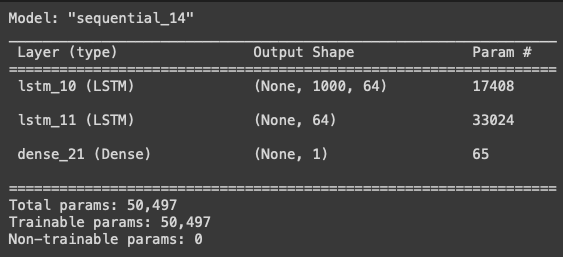
\includegraphics[width=.9\linewidth, height=4.5cm]{./images/model.png}
    }
    \caption{2-layer LSTM model architecture.}
    \label{fig:f3}
\end{figure}

%-------------------------------------------------------------------------
\section{Proposed Design}
\label{sec:design}

\textcolor{blue}{
    The device will be mounted on the ankle section of the patient and the test subjects. Acceleration data (together with other sensor data) will be collected and compared by the AI model~\cite[]{10.1007/978-3-319-59147-6_30}. Fully Connected Network (FCN) and LSTM will be used to evaluate which can better generate data from least data point and perform classification of whether the test subject has certain kinds of diseases that might cause walking gait issues. For example, there are results showing that FOG can be detected by just observing the walking gait of the test subject using a foot pressure sensor or accelerometer (Figure 4).
}

\begin{figure}[t]
    \centering
    \fbox{
        \rule{0pt}{2in} 
        \includegraphics[width=.9\linewidth, height=4.5cm]{./images/flowchart.png}
    }
    \caption{Flowchart of our proposed design.}
    \label{fig:f4}
\end{figure}

%-------------------------------------------------------------------------
\section{Future Work}
\label{sec:future_work}

\begin{itemize}
    \item \textcolor{blue}{Use InvenSense GY-521 MPU-6050 6DOF to generate Arduino powered Accelerometer.}
    \item \textcolor{blue}{Collect more patient-specific walking behaviors and use these data to train and test the model.}
    \item \textcolor{blue}{Calculate the accuracy and the loss function of the model.}
    \item \textcolor{blue}{Distinguish whether the test subjects have walking gait issues or not.}
    \item \textcolor{blue}{If it is difficult to classify whether the test subjects are abnormal or not, try to collect other information to improve the recognition.}
\end{itemize}

%-------------------------------------------------------------------------
\section{Expected results}
\label{sec:results}

A classification network that allows anyone to check their walking gait and provide feedback if an abnormality is detected.

%%%%%%%%% REFERENCES
{\small
\bibliographystyle{ieee_fullname}
\bibliography{egbib}
}

\end{document}
